\chapter{Remote Sensing Data and Geospatial Preprocessing}
\label{ch:preproc}

\chapmeta{Beginner $\to$ Intermediate}{$\sim$5\,h (2.5\,h + 2.5\,h)}{Sentinel-2 sample tiles; synthetic scenes}

\begin{objbox}
\begin{itemize}[leftmargin=1.2em,nosep]
  \item Read and write multi-band GeoTIFFs with \texttt{rasterio} and \texttt{rioxarray}.
  \item Understand CRS, geotransforms, and band resolution mismatches.
  \item Compute spectral indices (NDVI, NDWI, NDBI, EVI) as engineered channels.
  \item Choose and apply a normalization strategy for reflectance data.
  \item Tile a large scene into model-ready patches and reconstruct it.
\end{itemize}
\end{objbox}

This is the first genuinely Earth-Observation chapter: turning a raw
multispectral scene into tensors a CNN can train on. The steps --- loading,
index computation, normalization, tiling --- form the front half of every
pipeline in the rest of the book.

\section{Reading multi-band rasters}

A GeoTIFF couples a pixel grid with georeferencing: a CRS and an affine
\emph{geotransform} mapping array indices to world coordinates,
\begin{equation}
\begin{pmatrix}x\\y\end{pmatrix}
=\begin{pmatrix}a & b\\ d & e\end{pmatrix}\!\begin{pmatrix}\mathrm{col}\\ \mathrm{row}\end{pmatrix}
+\begin{pmatrix}c\\ f\end{pmatrix},
\end{equation}
where $(c,f)$ is the top-left corner and $a,e$ are the pixel sizes (with
$e<0$). \texttt{rasterio} exposes this as \texttt{src.transform} and the
projection as \texttt{src.crs}.
\begin{lstlisting}
import rasterio
with rasterio.open("scene.tif") as src:
    arr = src.read()          # (bands, H, W), native dtype (uint16 reflectance)
    profile = src.profile      # crs, transform, dtype, nodata, ...
\end{lstlisting}
\texttt{rioxarray} wraps the same data as a labelled \texttt{xarray.DataArray}
with named dimensions and coordinates, which is convenient for band maths and
resampling. A practical complication is that Sentinel-2 bands have \emph{mixed
resolutions} (10/20/60\,m); to stack them into one tensor you resample the
20/60\,m bands to the 10\,m grid (bilinear for continuous reflectance).

\section{Spectral indices as engineered features}

Normalised-difference indices are cheap, physically motivated channels that
often boost segmentation accuracy on the classes they target:
\begin{align}
\mathrm{NDVI} &= \frac{\mathrm{B08}-\mathrm{B04}}{\mathrm{B08}+\mathrm{B04}} &&\text{(vegetation)},\\
\mathrm{NDWI} &= \frac{\mathrm{B03}-\mathrm{B08}}{\mathrm{B03}+\mathrm{B08}} &&\text{(open water)},\\
\mathrm{NDBI} &= \frac{\mathrm{B11}-\mathrm{B08}}{\mathrm{B11}+\mathrm{B08}} &&\text{(built-up)},\\
\mathrm{EVI} &= 2.5\,\frac{\mathrm{B08}-\mathrm{B04}}{\mathrm{B08}+6\,\mathrm{B04}-7.5\,\mathrm{B02}+1} &&\text{(canopy, haze-robust)}.
\end{align}
Figure~\ref{fig:ndvi} shows a synthetic scene and its NDVI: forest and crops
light up, water goes negative. Appending such indices as extra channels gives
the network features it might otherwise have to learn from scratch.

\begin{figure}[h]
\centering
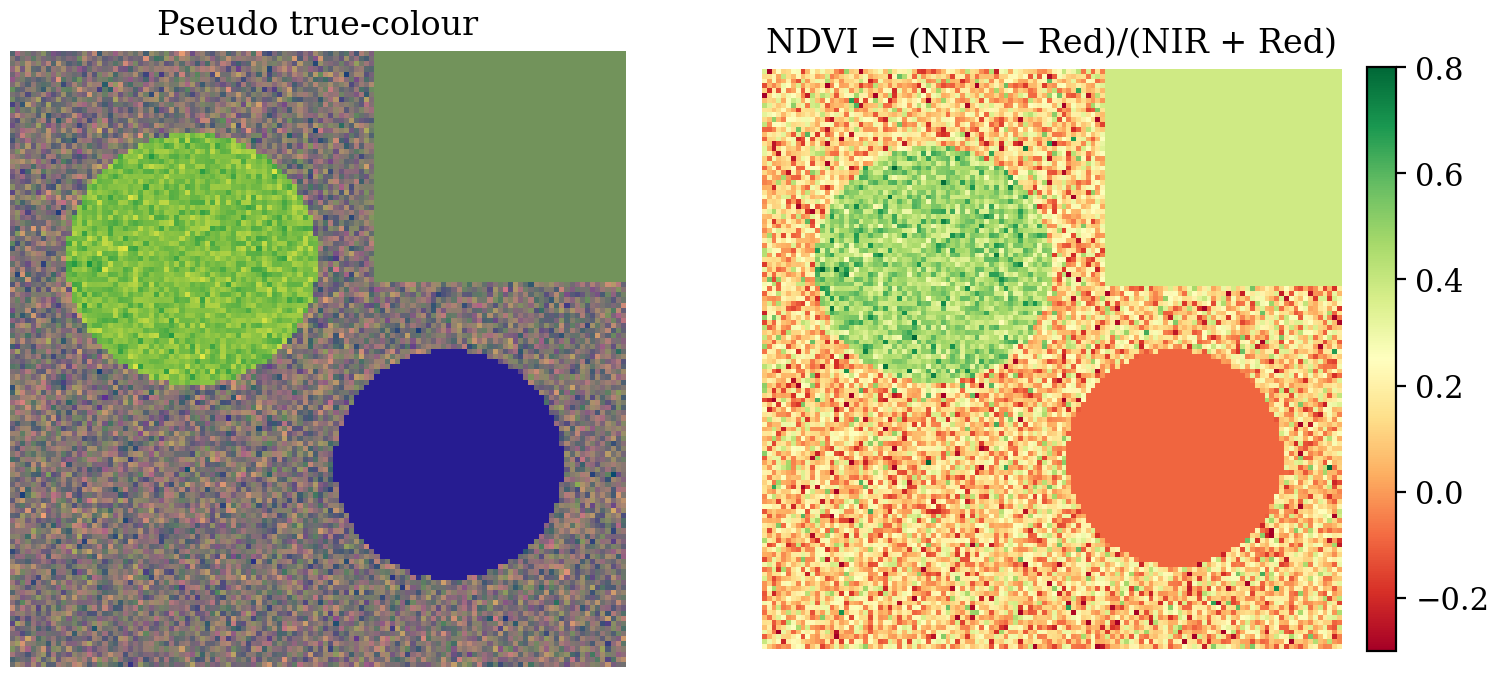
\includegraphics[width=0.86\linewidth]{figures/ndvi.png}
\caption{A pseudo true-colour scene (left) and its NDVI (right). High NDVI
(green) marks vegetation; water is strongly negative (red). Indices encode
domain knowledge as ready-made input channels.}
\label{fig:ndvi}
\end{figure}

\section{Normalization strategies}

Networks train best on inputs with comparable, $O(1)$ scales. Raw Sentinel-2
digital numbers span $0$--$10000$ and differ per band, so normalization is
mandatory (Figure~\ref{fig:norm}). Three common strategies:
\begin{description}[leftmargin=1.5em,style=nextline]
  \item[Min--max] $x'=(x-x_{\min})/(x_{\max}-x_{\min})\in[0,1]$. Simple but
  sensitive to outliers (a single bright cloud rescales everything).
  \item[Percentile clip] map the 2nd--98th percentile to $[0,1]$ and clip. Robust
  to outliers; the standard for visualisation and a strong default for training.
  \item[Z-score] $x'=(x-\mu_c)/\sigma_c$ with \emph{per-band} dataset statistics
  $\mu_c,\sigma_c$. Pairs naturally with ImageNet-pretrained encoders (which
  expect standardised inputs).
\end{description}

\begin{figure}[h]
\centering
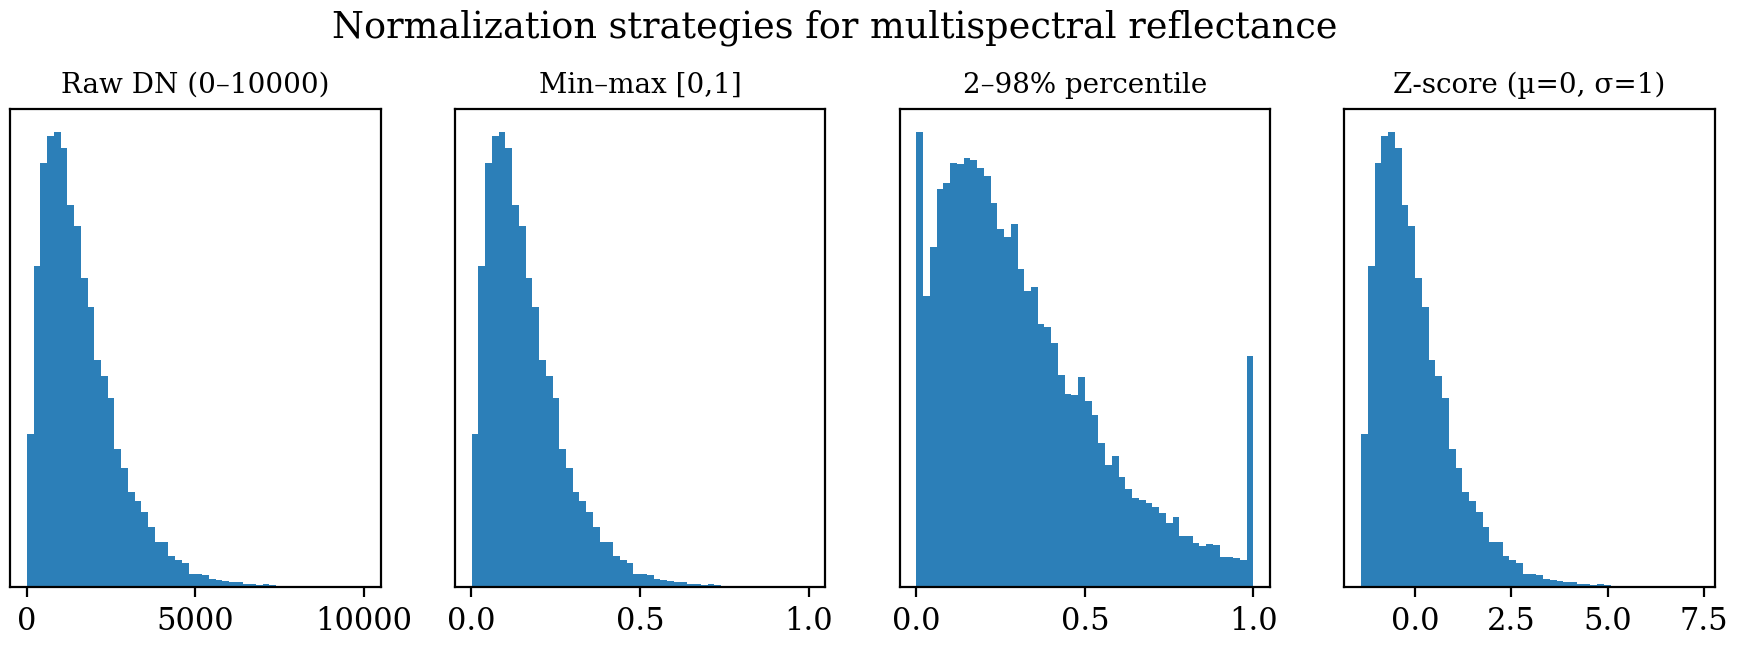
\includegraphics[width=\linewidth]{figures/normalization.png}
\caption{Effect of normalization on a reflectance histogram. Percentile clipping
tames the long bright tail; z-scoring centres each band at zero with unit
variance --- the form pretrained encoders expect.}
\label{fig:norm}
\end{figure}

\begin{notebox}[Train/serve consistency]
Compute normalization statistics on the \emph{training} set only and reuse them
unchanged for validation, test and inference. Recomputing per-image or per-split
statistics leaks information and breaks reproducibility in the deployed pipeline.
\end{notebox}

\section{Tiling a scene}

Sentinel-2 tiles are $\sim$$10980\times10980$ pixels --- far too large for a GPU.
We cut them into fixed patches (e.g.\ $512\times512$) with an overlap so that the
later sliding-window inference (Chapter~\ref{ch:pipeline}) can blend predictions
and avoid seams. Given tile size $T$ and stride $s<T$ (overlap $T-s$), tile
origins are $\{(i s, j s)\}$ clipped to the scene; edge tiles are padded.
Reconstruction reverses the process, accumulating predictions and dividing by a
weight map. A reusable preprocessing class typically chains: load $\to$ resample
$\to$ compute indices $\to$ normalize $\to$ tile, returning $(C,T,T)$ tensors
plus each tile's geotransform for georeferenced export later.

\begin{keybox}
\begin{itemize}[leftmargin=1.2em,nosep]
  \item GeoTIFF $=$ pixels $+$ CRS $+$ affine geotransform; read with \texttt{rasterio}/\texttt{rioxarray}.
  \item Resample mixed-resolution bands to a common grid before stacking.
  \item Spectral indices (NDVI/NDWI/NDBI/EVI) are cheap, informative extra channels.
  \item Normalize (percentile clip or per-band z-score) using \emph{training} statistics only.
  \item Tile large scenes with overlap; keep each tile's transform for export.
\end{itemize}
\end{keybox}

\begin{practbox}
Notebook: \nbpath{chapter\_04\_geospatial\_preprocessing/04\_practical\_sentinel2\_preprocessing.ipynb}.
\begin{enumerate}[leftmargin=1.4em,nosep]
  \item Generate (or download) a synthetic multi-band Sentinel-2 GeoTIFF; inspect
  shape, CRS, transform and per-band ranges with \texttt{rasterio}.
  \item Render true-colour and false-colour (NIR-Red-Green) composites.
  \item Load with \texttt{rioxarray}; compute NDVI and NDWI as new DataArrays.
  \item Compare min--max, percentile and z-score normalization via histograms.
  \item Implement \texttt{tile\_scene} / \texttt{reconstruct\_from\_tiles} and
  verify a round-trip reconstructs the input exactly.
\end{enumerate}
\begin{lstlisting}
def percentile_norm(band, lo=2, hi=98):
    p_lo, p_hi = np.percentile(band, [lo, hi])
    return np.clip((band - p_lo) / (p_hi - p_lo + 1e-6), 0, 1)
\end{lstlisting}
\end{practbox}

\begin{exbox}
\textbf{4.1 Real data.} Download a real Sentinel-2 L2A tile (e.g.\ via the
Copernicus browser or \texttt{sentinelsat}); load four 10\,m bands and resample
two 20\,m bands to 10\,m.\\[2pt]
\textbf{4.2 Index zoo.} Implement NDVI, NDWI, NDBI and EVI as functions; display
each over a real scene and interpret the highlighted land cover.\\[2pt]
\textbf{4.3 Overlap study.} Tile a scene at 0\%, 25\% and 50\% overlap; count
tiles and discuss the inference cost/quality trade-off.\\[2pt]
\textbf{Mini-project.} Build a \texttt{Sentinel2Tile} class that loads bands,
appends two indices, percentile-normalizes, and yields georeferenced
$512\times512$ tiles ready for a \texttt{DataLoader}.
\end{exbox}
